
\label{chap:implementation}
Our thesis work is split in three different projects: a refactoring of the already existing project\footnote{\hyperref[https://github.com/gibiansky/experiments/tree/master/nram]{https://github.com/gibiansky/experiments/tree/master/nram}} of Andrew Gibiansky, written in Python and based on Theano\footnote{Theano is a Python library created at LISA labs of University of Montreal, which lets to define easily complex mathematical expressions and execute them efficiently in the CPU and GPU specially with those which involves multi-dimensional arrays. The expressions definition is made through the creation of computational graph which is then executed and, if requested, automatic differentiated with an automatic differentiator, e.g. when one would calculate the gradient.} library, where some parts of NRAM and a parametrization system are missing, an implementation in C++ of the NRAM using DENN as optimization engine, and an additional implementation\footnote{\hyperref[https://github.com/DrugoLebowski/denn-lite-nram-executor]{https://github.com/DrugoLebowski/denn-lite-nram-executor}} of the NRAM used to test the generalization ability of the discovered ANNs.
\begin{figure}[h]
	\centering
	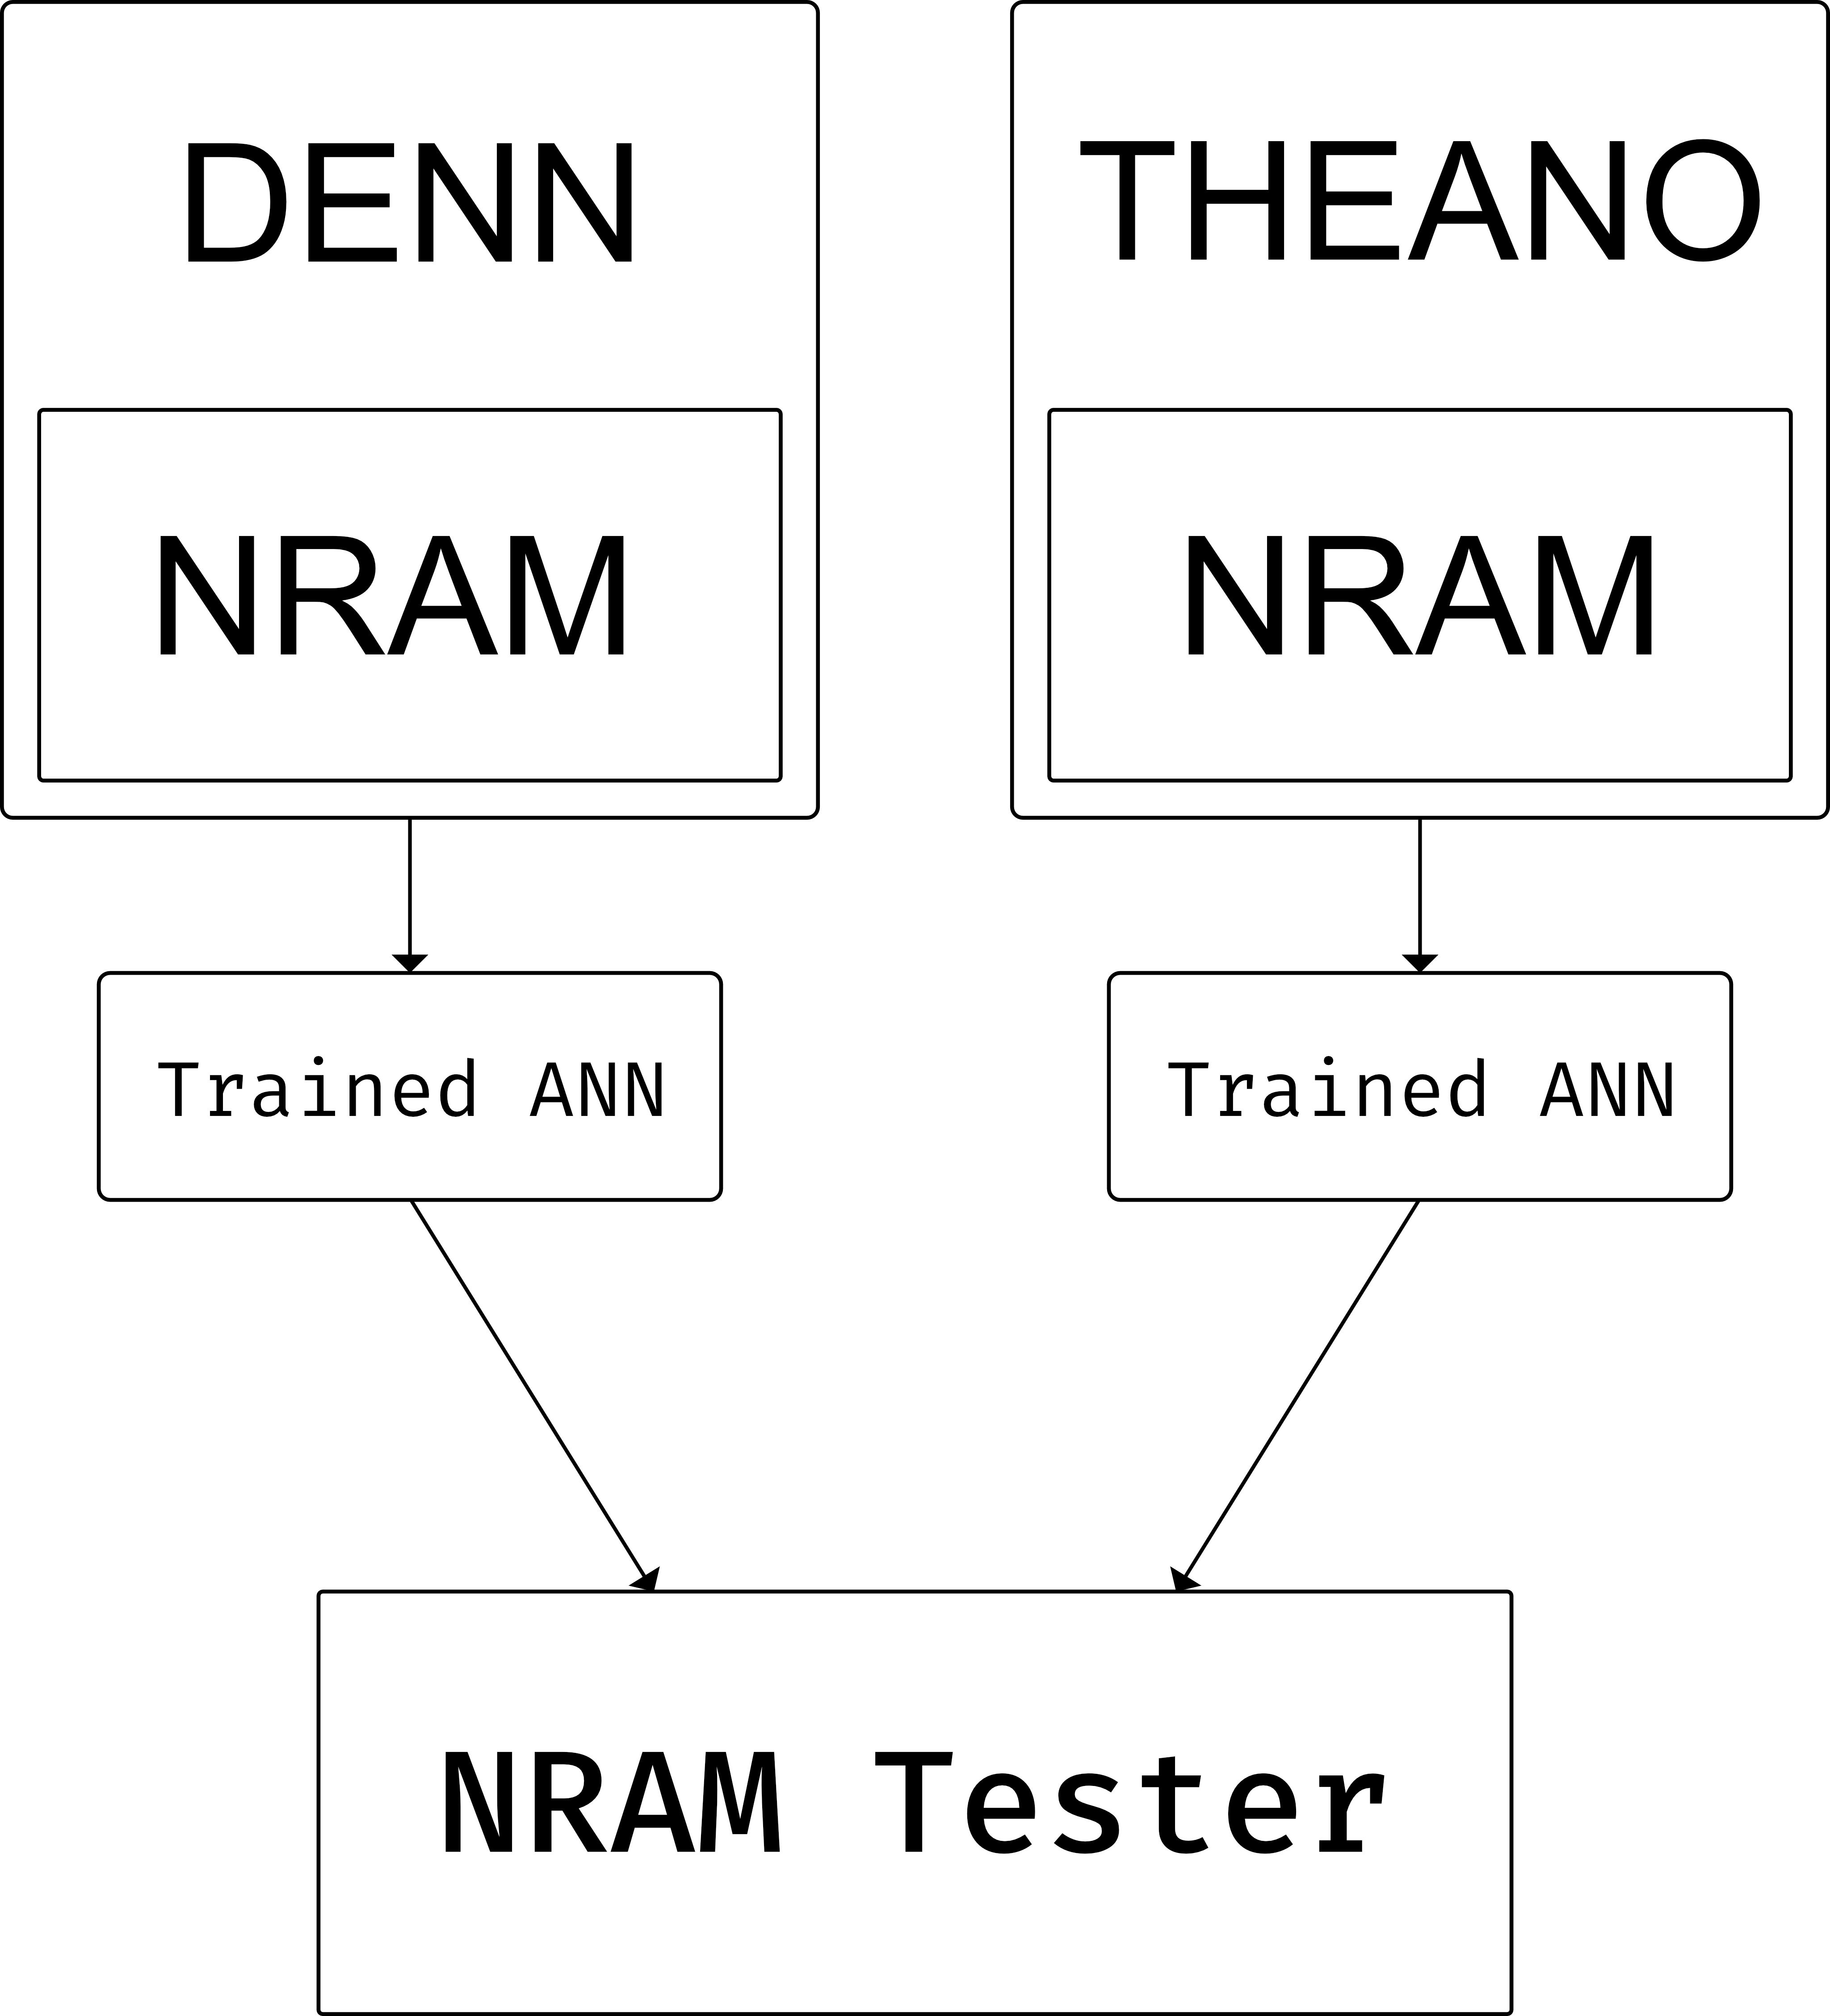
\includegraphics[width=0.5\linewidth]{figures/NRAM-implementation.png}
	\caption{System structure: the first two blocks are the implementations used to train the neural networks. Once a controller is trained, it can be run with the NRAM Tester, i.e. the \textit{vanilla} version without the training phase, to test the generalization ability and to visualize the produced circuits.}
	\label{fig:nram-implementation-scheme}
\end{figure}

\paragraph{Preface}
Since some of the tasks presented in Chapter \ref{experiments} are too complex to be learned by a plain NRAM, we have also used some of the enhanchements described in \cite{NRAM:2016}.

\subparagraph{Gradient clipping}
The size of the model can be extremely large and moreover extremely depth, due to the execution in various timesteps. In these types of networks the gradient can often explode, as noticed in \cite{Bengio1994LearningLD}. Hence, in the Theano implementation all the gradients are clipped in the range $[-C_1, C_1]$ and successively rescaled, such that its $L_2$ norm\footnote{Let $\textbf{x} = [x_1, x_2, \dots, x_n]$, the norm $L_2$ is defined as $|\textbf{x}| = \sqrt{\sum\limits_{k=1}^{n}|x_i|^2}$.} is not larger than some constant $C_2$.

\subparagraph{Noise}
As noticed in \cite{Neelakantan2015AddingGN}, in the Theano implementation a Gaussian noise, whose variance decays over times, is added to the computed gradient.

\subparagraph{Entropy}
As for \cite{NRAM:2016}, we also noticed that the network can fix the registers used as pointers in some value. Although it could be an advantage in some cases, if this happens too early in the training phase, it could force the network to stay fixed on some pointer with a very small chances of change. Hence, to alleviate this condition, we give to the network a sort of a ``entropy bonus'' which decreases over time. This entropy is computed for each generated distribution\footnote{We have identified these distributions be those in the memory.} by the neural network with the Shannon entropy and is multiplied by the following coefficient that decreases over time
\begin{equation}
	E = e * d^{t}
\end{equation}
where $e$ is the entropy coefficient, $d$ is the decay of the entropy coefficient and $t$ is the timestep. After that, the computed value is subtracted from the cost of the timestep $t$ (Please refer to Section \ref{subsec:cost-function} to see how the cost is computed).

\subparagraph{Curriculum learning}\label{subpar:curriculum-learning}
As noticed by \cite{Bengio2009CurriculumL} and \cite{Zaremba2014LearningTE}, curriculum learning is crucial to train very deep neural networks. Hence, as in the original paper, we decided to implement in the system the curriculum learning described in \cite{Zaremba2014LearningTE}.

For each task, we have defined manually a set of problems of increasing difficulties, where the difficulty $d$ is defined as a tuple containing the length of the working sequence and the number of timesteps of running. During the training, a difficulty tuple is selected according to the current difficulty $D$ as follows:
\begin{itemize}
	\item{with probability 10\%: pick $d$ randomly from the set of all difficulties according to a uniform distribution.}
	\item{with probability 25\%: pick $d$ randomly from the set $[1, D + e]$ according to a uniform distribution, with $e$ is generated from a geometric distribution with a success probability of 0.5.}
	\item{with probability 65\%: set $d = D + e$ where $e$ is sampled as above.}
\end{itemize}
The difficulty is increased when $1 - \frac{c}{m} < \lambda$. $1 - \frac{c}{m}$ is the error rate, $c$ represents the correct modified cells, $m$ the cells that should be modified and $\lambda$ is a threshold chosen by the user. Furthermore, we ensure that the difficulty is increased again at least after a given number of generations.


\section{How we did it}
The implementation of NRAM module is similar both in DENN and Theano versions, differentiating only for the training algorithm and for some specific technique (for example, Gradient Clipping is useless in the implementation with DENN and so it is not implemented). Hence, leaving out these specifics of the framework we speak only about the NRAM implementation which is presented for simplicity as pseudocode\footnote{The entire code is available at \href{https://github.com/Gabriele91/DENN-LITE/tree/nram}{https://github.com/Gabriele91/DENN-LITE/tree/nram}}.\newline
The main block of NRAM can be seen in Algorithm \ref{alg:nram-main-block}. The execution starts with the setting of some variables, such as cost variable and the constants used for the computing of the entropy. The main cycle is at Line \ref{lst:nram-timesteps} - in every timestep the network releases all the coefficients, i.e. the circuit connections, at Line \ref{lst:nram-nn-predict}. At Line \ref{lst:nram-run-circuit} is executed the circuit, with the Algorithm \ref{alg:nram-run-circuit} - it returns the willingness of terminate the execution with which is computed from Line \ref{lst:nram-cost-1} to \ref{lst:nram-cost-2} the timestep cost, added later to the total cost. At Line \ref{lst:willingness-terminate}, if the willingness of terminate reaches the value $1.0$ then the execution of the NRAM is terminated. The ``magic'' of NRAM happens in Algorithm \ref{alg:nram-run-circuit}, where the circuit is executed. From Line \ref{lst:nram-exec-circuit-1} to \ref{lst:nram-exec-circuit-2}, each gate in the list \textbf{Gates} is executed, getting an input\footnote{Depending by the type - Costant gate produce a constant output without getting an input, unary and binary gate gate get, respectively, one and two input.} and producing an output, which might be accessed later by another gate or register. From Line \ref{lst:nram-up-reg-1} to \ref{lst:nram-up-reg-2}, the registers are updated. As it can be seen in the Lines \ref{lst:nram-avg-1}, \ref{lst:nram-avg-2}, \ref{lst:nram-avg-3} and \ref{lst:nram-avg-4}, the selection of the input of a gate and the new content of the register is made through the function in the Algorithm \ref{alg:nram-average} which do a weighted average. An example of gate is visible in Algorithm \ref{alg:nram-gate-add} - the \textbf{add} gate compute the summation of two number represented as two probability distributions. Finally, the functions \textsc{GetGateCoefficient} and \textsc{GetRegisterCoefficient} are purely conceptual functions which indicates a method with which the coefficients are acquired.

The pseudocode of the implementation of the NRAM used to test the generalization ability of the discovered ANNs is showed in Algorithm \ref{alg:nram-main-block-test}. For each test, defined by the size of the memory and the timesteps, is executed the NRAM for each sample - with the results at Line \ref{lst:nram-test-print-circuit} is written to file the circuits generated during the execution. At Line \ref{lst:nram-test-print-memories} and at Line \ref{lst:nram-test-print-error-rate}, when all the samples of a difficulty are managed, are printed to an image the memories and to a csv the error rate reached by NRAM for the current difficulty. 

\subsection{Datasets}\label{subsubsec:nram-dataset}
The datasets used during the training are automatically generated at runtime. Each batch of samples is composed by:
\begin{itemize}
	\item{initial memories: the memories which are manipulated by NRAM during the execution;}
	\item{expected memories: the memories which are compared to the modified initial memories for cost computation;}
	\item{cost masks: used to take into account only parts of the memories during the computing of the cost;}
	\item{error rate masks: used to take into account only parts of the memories during the computing of the error rate;}
\end{itemize}
Remembering how a classification problem is defined, from an high level the $x$ is formed by the Registers and ``Initial memory'' and the $y$ is the ``Expected Memory''. The datasets are generated only at the beginning of the training of the NRAM, except when the Curriculum Learning is active in which are re-generated to every change of difficulty.

\begin{algorithm}
	\begin{algorithmic}[1]
		\Function{NRAM}{NeuralNetwork, BatchSize, Regs, IMem, OMem, CostMask, MaxInt, T, Gates}
			\State{Cost = 0.0}			
            	\State{ProbIncomplete = 1.0}
            	\State{CumProbComplete = 0.0};
            	\State{$p_T = 1.0$}
            	\State{EntropyCoeff = 0.1}
            	\State{EntropyDecay = 0.999}
			\For{$t\in[1, \dots, T]$}\label{lst:nram-timesteps}
				\State{Conf = \Call{NeuralNetwork.predict(Regs.ProbZero())}{}}\label{lst:nram-nn-predict}
				\State{$\{f_i, \textrm{Regs}, \textrm{IMem}\}$ = \Call{RunCircuit}{Gates, Conf, Regs, IMem, MaxInt}}\label{lst:nram-run-circuit}
				\State{}
				\If{t == T}\label{lst:nram-cost-1}
					\State{$p_T$ = 1 - CumProbComplete}
				\Else
					\State{$p_T$ = $f_i$ * ProbIncomplete}
				\EndIf
				\State{}
               	\State{CumProbComplete = CumProbComplete + $p_t$}
                	\State{ProbIncomplete = ProbIncomplete * ($1 - f_i$)}
				\State{}
                	\State{EntropyWeight = $\textrm{EntropyCoeff}*\textrm{EntropyDecay}^t$}
                	\State{EntropyCost = EntropyCost+\Call{Entropy}{IMem} * EntropyWeight}
				\State{}
                	\State{Cost += \Call{CalculateCost}{InMem, OutMem, CostMask} - EntropyCost}\label{lst:nram-cost-2}
                	
                	\If{$f_i \geq 1.0$}\label{lst:willingness-terminate}
                		\State{break}
                	\EndIf
			\EndFor{}
			\State{}
			\State{\Return Cost}
		\EndFunction
	\end{algorithmic}
	\caption{Pseudocode of the main block of NRAM.}\label{alg:nram-main-block}
\end{algorithm}

\begin{algorithm}
	\begin{algorithmic}[1]
		\Function{RunCircuit}{Gates, Conf, Regs, IMem, MaxInt}
			\State{RegsAndOutput = \Call{Copy}{Regs}}
			\State{}
			\ForEach{$g\in \textrm{Gates}$}\Comment{Run of the circuit}\label{lst:nram-exec-circuit-1}
				\If{\Call{g.isConstant}}
					\State{GateResult = g.\Call{Value}{}}
				\ElsIf{\Call{g.isUnary}}
					\State{Coeff = \Call{GetGateCoefficient}{Conf, g}}
					\State{InputValue = \Call{Avg}{RegsAndOutput, Coeff}}\label{lst:nram-avg-1}
					\State{GateResult = g.\Call{execute}{InputValue, IMem, MaxInt}}	
				\Else
					\State{(CoeffA, CoeffB) = \Call{GetGateCoefficient}{Conf, g}}
					\State{InputValueA = \Call{Avg}{RegsAndOutput, CoeffA}}\label{lst:nram-avg-2}
					\State{InputValueB = \Call{Avg}{RegsAndOutput, CoeffB}}\label{lst:nram-avg-3}
					\State{GateResult = g.\Call{execute}{GateValueA, GateValueB, IMem, MaxInt}}	
				\EndIf
				\State{RegsAndOutput = \Call{Concatenate}{Regs, GateValue}}
			\EndFor{}\label{lst:nram-exec-circuit-2}
			\newline
			\For{$i\in[1, \dots, |\textrm{Regs}|]$}\Comment{Update of the registers}\label{lst:nram-up-reg-1}
				\State{Coeff = \Call{GetGateCoefficient}{Conf, i}}
				\State{NewValue = \Call{Avg}{RegsAndOutput, Coeff}}\label{lst:nram-avg-4}
				\State{Regs[i] = NewValue}
			\EndFor{}\label{lst:nram-up-reg-2}
			\State{}
			\State{\Return{(Conf[\Call{Conf.size} - 1], Regs, IMem)}}
		\EndFunction
	\end{algorithmic}
	\caption{Pseudocode of the run circuit function.}\label{alg:nram-run-circuit}
\end{algorithm}


\begin{algorithm}
	\begin{algorithmic}[1]
		\Function{Avg}{RegsOut, Coefficient} 
			\State{\Return{RegsOut * Coefficient}}
		\EndFunction
	\end{algorithmic}
	\caption{Pseudocode of the avg function}\label{alg:nram-average}
\end{algorithm}

\begin{algorithm}
	\begin{algorithmic}[1]
		\Function{Add}{A, B, IMem, MaxInt}
			\State{C = \Call{Zero(MaxInt)}{}}\Comment{Matrix of zeros where is stored the output of the module Add} 
			\For{$i \in [0, \textrm{MaxInt} - 1]$}
				\For{$j \in [0, \textrm{MaxInt} - 1]$}
					\State{C[j] += A[i] * B[(j - i) \% MaxInt]}
				\EndFor{}
			\EndFor{}
			\State{\Return{C}}
		\EndFunction
	\end{algorithmic}
	\caption{Example of NRAM gate.}
	\label{alg:nram-gate-add}
\end{algorithm}

\begin{algorithm}
	\begin{algorithmic}[1]
		\Function{NramTest}{NeuralNetwork, BatchSize, Tests, Gates}
			\For{$\{$MaxInt, Timestep$\} \in $Tests}
				\State{$\{$Regs, IMem, OMem, CostMask$\}$ = \Call{GenerateBatch}{BatchSize, MaxInt, Timestep}}
				\For{$s \in [1, \dots, $BatchSize$]$}
					\State{SampleIMem = IMem[s]}
					\State{SampleOMem = OMem[s]}
					\State{SampleRegs = Regs[s]}
					\For{$t \in [1, \dots, $Timestep$]$}
						\State{Conf = \Call{NeuralNetwork.predict}{Regs.ProbZero()}}
						\State{$\{$SampleRegs, SampleIMem$\}$ = \Call{RunCircuit}{Gates, Conf, SampleRegs, SampleIMem, MaxInt}}
					 	\State{\Call{PrintCircuitToFile}{Conf}}\label{lst:nram-test-print-circuit}
					\EndFor{}
				\EndFor{}
				\State{\Call{PrintMemoriesToFile}{SampleIMem}}\label{lst:nram-test-print-memories}
				\State{\Call{PrintErrorRateToFile}{SampleIMem, SampleOMem, CostMask}}\label{lst:nram-test-print-error-rate}
			\EndFor{}
		\EndFunction
	\end{algorithmic}
	\caption{Pseudocode of the NRAM tester.}\label{alg:nram-main-block-test}
\end{algorithm}